\documentclass[border=8pt]{standalone}
\usepackage{amsmath}
\usepackage{amssymb}
\usepackage{tikz}
\usetikzlibrary{arrows.meta,calc,decorations.pathreplacing,patterns,shapes.geometric,positioning,shadings,plotmarks}

\definecolor{panelbg}{RGB}{250,247,240}
\definecolor{softgrey}{RGB}{95,90,85}
\definecolor{darkgold}{RGB}{140,95,20}
\definecolor{fitred}{RGB}{190,40,40}
\definecolor{fitblue}{RGB}{30,90,170}
\definecolor{axiscol}{RGB}{60,55,50}

\begin{document}
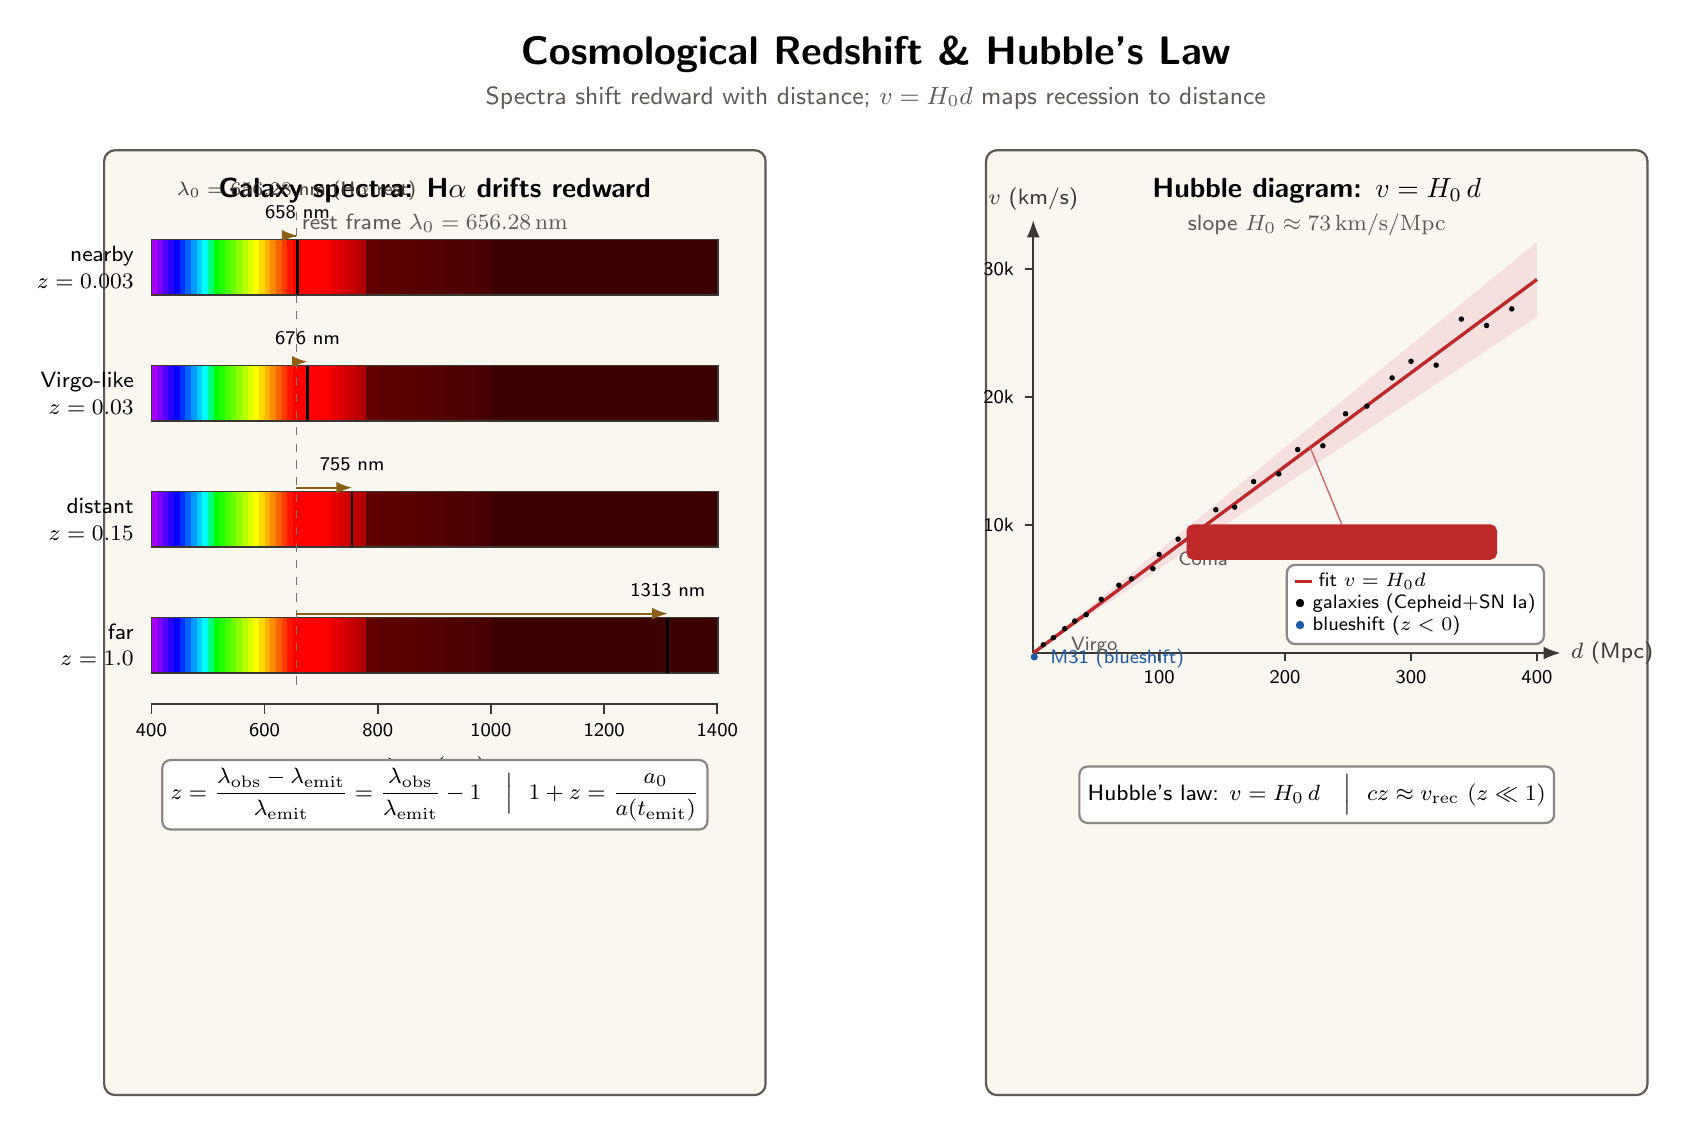
\begin{tikzpicture}[
  font=\sffamily,
  axisstyle/.style={line width=0.8pt,axiscol,-{Latex[length=2.2mm]}},
  fitline/.style={line width=1.2pt,fitred},
  tickstyle/.style={line width=0.6pt,axiscol},
  spectrumbox/.style={draw=axiscol,line width=0.6pt},
  arr/.style={-{Latex[length=2mm]},line width=0.7pt},
]

% ============================================================
% TITLE
% ============================================================
\node[font=\sffamily\bfseries\Large] at (0,9.6) {Cosmological Redshift \& Hubble's Law};
\node[font=\sffamily\small,softgrey] at (0,9.05) {Spectra shift redward with distance; $v = H_0 d$ maps recession to distance};

% ============================================================
% LEFT PANEL: Four spectra with Halpha line shifting redward
% ============================================================
\node[rounded corners=4pt,draw=softgrey,fill=panelbg,thick,
      minimum width=84mm,minimum height=120mm,anchor=north] at (-5.6,8.4) {};

\node[font=\sffamily\bfseries,anchor=north] at (-5.6,8.15) {Galaxy spectra: H$\alpha$ drifts redward};
\node[font=\sffamily\footnotesize,softgrey,anchor=north] at (-5.6,7.7) {rest frame $\lambda_0 = 656.28\,\mathrm{nm}$};

% Wavelength axis: 400 to 1400 nm, x in [-9.2, -2.0]
\def\xmin{-9.2}
\def\xmax{-2.0}
\def\lmin{400}
\def\lmax{1400}
\pgfmathsetmacro{\xscale}{(\xmax-\xmin)/(\lmax-\lmin)}

% Y positions of spectra
\def\yA{6.9}
\def\yB{5.3}
\def\yC{3.7}
\def\yD{2.1}
\def\spheight{0.7}

% Gradient macro using many thin rectangles with interpolated RGB colors
\newcommand{\drawspectrum}[1]{%
  \foreach \wl in {400,410,...,1390}{%
    \pgfmathtruncatemacro{\wlnext}{\wl+10}
    \pgfmathsetmacro{\xA}{\xmin + (\wl-\lmin)*\xscale}
    \pgfmathsetmacro{\xB}{\xmin + (\wlnext-\lmin)*\xscale}
    \pgfmathtruncatemacro{\wlf}{\wl}
    \pgfmathsetmacro{\R}{
      (\wlf<380)*0 +
      (\wlf>=380 && \wlf<440)*(-(\wlf-440)/60) +
      (\wlf>=440 && \wlf<510)*0 +
      (\wlf>=510 && \wlf<580)*((\wlf-510)/70) +
      (\wlf>=580 && \wlf<645)*1 +
      (\wlf>=645 && \wlf<780)*1 +
      (\wlf>=780)*0.6
    }
    \pgfmathsetmacro{\G}{
      (\wlf<380)*0 +
      (\wlf>=380 && \wlf<440)*0 +
      (\wlf>=440 && \wlf<490)*((\wlf-440)/50) +
      (\wlf>=490 && \wlf<580)*1 +
      (\wlf>=580 && \wlf<645)*(-(\wlf-645)/65) +
      (\wlf>=645)*0
    }
    \pgfmathsetmacro{\B}{
      (\wlf<380)*0 +
      (\wlf>=380 && \wlf<440)*1 +
      (\wlf>=440 && \wlf<490)*1 +
      (\wlf>=490 && \wlf<510)*(-(\wlf-510)/20) +
      (\wlf>=510)*0
    }
    \pgfmathsetmacro{\Rc}{max(0,min(1,\R))}
    \pgfmathsetmacro{\Gc}{max(0,min(1,\G))}
    \pgfmathsetmacro{\Bc}{max(0,min(1,\B))}
    \pgfmathsetmacro{\fF}{
      (\wlf<700)*1 +
      (\wlf>=700 && \wlf<780)*(1-(\wlf-700)/200) +
      (\wlf>=780 && \wlf<1000)*(0.55-(\wlf-780)*0.0010) +
      (\wlf>=1000)*0.25
    }
    \pgfmathsetmacro{\fFc}{max(0.10,min(1,\fF))}
    \pgfmathsetmacro{\Rf}{\Rc*\fFc + (1-\fFc)*0.12}
    \pgfmathsetmacro{\Gf}{\Gc*\fFc}
    \pgfmathsetmacro{\Bf}{\Bc*\fFc}
    \definecolor{tmpcol}{rgb}{\Rf,\Gf,\Bf}
    \fill[tmpcol] (\xA,#1-\spheight/2) rectangle (\xB,#1+\spheight/2);
  }
}

% Draw four spectrum bands
\drawspectrum{\yA}
\drawspectrum{\yB}
\drawspectrum{\yC}
\drawspectrum{\yD}

% Borders
\foreach \yc in {\yA,\yB,\yC,\yD}{
  \draw[spectrumbox] (\xmin,\yc-\spheight/2) rectangle (\xmax,\yc+\spheight/2);
}

% Rest-frame reference line at 656.28 nm
\pgfmathsetmacro{\xrest}{\xmin + (656.28-\lmin)*\xscale}
\draw[dashed,line width=0.6pt,axiscol!70]
  (\xrest,\yD-\spheight/2-0.15) -- (\xrest,\yA+\spheight/2+0.35);
\node[font=\sffamily\scriptsize,axiscol,anchor=south] at (\xrest,\yA+\spheight/2+0.38) {$\lambda_0=656.28$ nm (H$\alpha$ rest)};

% Observed Halpha lines (black) for each z
% z = 0.003, 0.03, 0.15, 1.0  -> lobs = 658.25, 675.97, 754.72, 1312.56
\pgfmathsetmacro{\xAobs}{\xmin + (658.25-\lmin)*\xscale}
\draw[line width=1.0pt,black] (\xAobs,\yA-\spheight/2) -- (\xAobs,\yA+\spheight/2);

\pgfmathsetmacro{\xBobs}{\xmin + (675.97-\lmin)*\xscale}
\draw[line width=1.0pt,black] (\xBobs,\yB-\spheight/2) -- (\xBobs,\yB+\spheight/2);

\pgfmathsetmacro{\xCobs}{\xmin + (754.72-\lmin)*\xscale}
\draw[line width=1.0pt,black] (\xCobs,\yC-\spheight/2) -- (\xCobs,\yC+\spheight/2);

\pgfmathsetmacro{\xDobs}{\xmin + (1312.56-\lmin)*\xscale}
\draw[line width=1.0pt,black] (\xDobs,\yD-\spheight/2) -- (\xDobs,\yD+\spheight/2);

% Shift arrows above each spectrum
\draw[arr,darkgold] (\xrest,\yA+\spheight/2+0.05) -- (\xAobs,\yA+\spheight/2+0.05);
\draw[arr,darkgold] (\xrest,\yB+\spheight/2+0.05) -- (\xBobs,\yB+\spheight/2+0.05);
\draw[arr,darkgold] (\xrest,\yC+\spheight/2+0.05) -- (\xCobs,\yC+\spheight/2+0.05);
\draw[arr,darkgold] (\xrest,\yD+\spheight/2+0.05) -- (\xDobs,\yD+\spheight/2+0.05);

% Labels at left of each spectrum
\node[font=\sffamily\footnotesize,anchor=east,align=right] at (\xmin-0.1,\yA) {nearby\\$z=0.003$};
\node[font=\sffamily\footnotesize,anchor=east,align=right] at (\xmin-0.1,\yB) {Virgo-like\\$z=0.03$};
\node[font=\sffamily\footnotesize,anchor=east,align=right] at (\xmin-0.1,\yC) {distant\\$z=0.15$};
\node[font=\sffamily\footnotesize,anchor=east,align=right] at (\xmin-0.1,\yD) {far\\$z=1.0$};

% Observed wavelength labels above each obs line
\node[font=\sffamily\scriptsize,anchor=south] at (\xAobs,\yA+\spheight/2+0.15) {658 nm};
\node[font=\sffamily\scriptsize,anchor=south] at (\xBobs,\yB+\spheight/2+0.15) {676 nm};
\node[font=\sffamily\scriptsize,anchor=south] at (\xCobs,\yC+\spheight/2+0.15) {755 nm};
\node[font=\sffamily\scriptsize,anchor=south] at (\xDobs,\yD+\spheight/2+0.15) {1313 nm};

% Wavelength axis below bottom spectrum
\def\yaxis{1.35}
\draw[line width=0.7pt,axiscol] (\xmin,\yaxis) -- (\xmax,\yaxis);
\foreach \wl in {400,600,800,1000,1200,1400}{
  \pgfmathsetmacro{\xtick}{\xmin + (\wl-\lmin)*\xscale}
  \draw[tickstyle] (\xtick,\yaxis) -- (\xtick,\yaxis-0.12);
  \node[font=\sffamily\scriptsize,anchor=north] at (\xtick,\yaxis-0.12) {\wl};
}
\node[font=\sffamily\footnotesize,anchor=north,axiscol] at ({(\xmin+\xmax)/2},\yaxis-0.55) {$\lambda_{\mathrm{obs}}$ (nm)};

% Formula (1) below left panel
\node[rounded corners=3pt,draw=axiscol!60,fill=white,thick,inner sep=3pt,
      font=\sffamily\footnotesize,align=center] at (-5.6,0.2)
  {$z = \dfrac{\lambda_{\mathrm{obs}}-\lambda_{\mathrm{emit}}}{\lambda_{\mathrm{emit}}}
   = \dfrac{\lambda_{\mathrm{obs}}}{\lambda_{\mathrm{emit}}}-1$
   \ \ $\Big|$\ \
   $1+z = \dfrac{a_0}{a(t_{\mathrm{emit}})}$};

% ============================================================
% RIGHT PANEL: Hubble diagram v vs d
% ============================================================
\node[rounded corners=4pt,draw=softgrey,fill=panelbg,thick,
      minimum width=84mm,minimum height=120mm,anchor=north] at (5.6,8.4) {};

\node[font=\sffamily\bfseries,anchor=north] at (5.6,8.15) {Hubble diagram: $v = H_0\, d$};
\node[font=\sffamily\footnotesize,softgrey,anchor=north] at (5.6,7.7) {slope $H_0 \approx 73\,\mathrm{km/s/Mpc}$};

% Plot region
% Use distance in Mpc and velocity in units of (1000 km/s = Mm/s) to keep numbers small
\def\xO{2.0}
\def\yO{2.0}
\def\xend{8.4}
\def\yend{7.2}
\def\dMaxM{400}
\def\vMaxU{32}   % 32 units = 32000 km/s
\pgfmathsetmacro{\xpscale}{(\xend-\xO)/(\dMaxM)}
\pgfmathsetmacro{\ypscale}{(\yend-\yO)/(\vMaxU)}
% Slope: v(km/s) = 73*d(Mpc); in units v_u = 0.073*d

% Axes
\draw[axisstyle] (\xO,\yO) -- (\xend+0.3,\yO) node[right,font=\sffamily\footnotesize,axiscol] {$d$ (Mpc)};
\draw[axisstyle] (\xO,\yO) -- (\xO,\yend+0.3) node[above,font=\sffamily\footnotesize,axiscol] {$v$ (km/s)};

% X-ticks
\foreach \d/\lbl in {100/100,200/200,300/300,400/400}{
  \pgfmathsetmacro{\xt}{\xO + \d*\xpscale}
  \draw[tickstyle] (\xt,\yO) -- (\xt,\yO-0.1);
  \node[font=\sffamily\scriptsize,anchor=north] at (\xt,\yO-0.1) {\lbl};
}

% Y-ticks (labels in km/s)
\foreach \vu/\lbl in {10/10k,20/20k,30/30k}{
  \pgfmathsetmacro{\yt}{\yO + \vu*\ypscale}
  \draw[tickstyle] (\xO,\yt) -- (\xO-0.1,\yt);
  \node[font=\sffamily\scriptsize,anchor=east] at (\xO-0.12,\yt) {\lbl};
}

% Shaded +-10% band (using velocity in thousand-km/s units)
\pgfmathsetmacro{\xLineMax}{\xO + \dMaxM*\xpscale}
\pgfmathsetmacro{\vAtMaxU}{0.073*\dMaxM}
\pgfmathsetmacro{\yBandHi}{\yO + 1.10*\vAtMaxU*\ypscale}
\pgfmathsetmacro{\yBandLo}{\yO + 0.90*\vAtMaxU*\ypscale}
\fill[fitred!15]
  (\xO,\yO) -- (\xLineMax,\yBandHi) -- (\xLineMax,\yBandLo) -- cycle;

% Hubble line
\pgfmathsetmacro{\yLineMax}{\yO + \vAtMaxU*\ypscale}
\draw[fitline] (\xO,\yO) -- (\xLineMax,\yLineMax);

% Data points scattered around v = 73 d within ~+-10%; velocities in thousand-km/s units
\foreach \d/\vu in {
  8/0.65,
  16/1.20,
  25/1.90,
  33/2.50,
  42/3.00,
  54/4.20,
  68/5.30,
  78/5.80,
  95/6.60,
  100/7.70,
  115/8.90,
  130/9.10,
  145/11.20,
  160/11.40,
  175/13.40,
  195/14.00,
  210/15.90,
  230/16.20,
  248/18.70,
  265/19.30,
  285/21.50,
  300/22.80,
  320/22.50,
  340/26.10,
  360/25.60,
  380/26.90}{
  \pgfmathsetmacro{\xpt}{\xO + \d*\xpscale}
  \pgfmathsetmacro{\ypt}{\yO + \vu*\ypscale}
  \fill[black] (\xpt,\ypt) circle (1.0pt);
}

% Andromeda blueshift (negative velocity: -300 km/s = -0.3 units)
\pgfmathsetmacro{\xAnd}{\xO + 0.8*\xpscale}
\pgfmathsetmacro{\yAnd}{\yO + (-0.30)*\ypscale}
\fill[fitblue] (\xAnd,\yAnd) circle (1.3pt);
\node[font=\sffamily\scriptsize,fitblue,anchor=west] at (\xAnd+0.08,\yAnd-0.02) {M31 (blueshift)};

% Virgo (16 Mpc, 1200 km/s), Coma (100 Mpc, 7700 km/s)
\pgfmathsetmacro{\xVirgo}{\xO + 16*\xpscale}
\pgfmathsetmacro{\yVirgo}{\yO + 1.20*\ypscale}
\node[font=\sffamily\scriptsize,softgrey,anchor=west] at (\xVirgo+0.1,\yVirgo-0.1) {Virgo};

\pgfmathsetmacro{\xComa}{\xO + 100*\xpscale}
\pgfmathsetmacro{\yComa}{\yO + 7.70*\ypscale}
\node[font=\sffamily\scriptsize,softgrey,anchor=west] at (\xComa+0.12,\yComa-0.05) {Coma};

% Slope label near the line
\pgfmathsetmacro{\xMid}{\xO + 220*\xpscale}
\pgfmathsetmacro{\yMid}{\yO + 0.073*220*\ypscale}
\node[rounded corners=2pt,draw=fitred,fill=white,thick,
      font=\sffamily\footnotesize,fitred,inner sep=2pt]
  (slp) at (\xMid+0.4,\yMid-1.2) {$v = H_0 d,\ H_0\!\approx\!73\,\mathrm{km/s/Mpc}$};
\draw[line width=0.5pt,fitred!70] (slp.north) -- (\xMid,\yMid);

% Legend
\node[rounded corners=3pt,draw=axiscol!60,fill=white,thick,inner sep=3pt,
      font=\sffamily\scriptsize,align=left,anchor=south east]
  at (8.5,2.1)
  {\textcolor{fitred}{\rule[0.4ex]{6pt}{1.0pt}} fit $v=H_0 d$ \\
   \textbullet\ galaxies (Cepheid$+$SN Ia) \\
   \textcolor{fitblue}{\textbullet}\ blueshift ($z<0$)};

% Formula (3) under right panel
\node[rounded corners=3pt,draw=axiscol!60,fill=white,thick,inner sep=3pt,
      font=\sffamily\footnotesize,align=center] at (5.6,0.2)
  {Hubble's law: $v = H_0\, d$
   \ \ $\Big|$\ \
   $cz \approx v_{\mathrm{rec}}\ (z\ll 1)$};

\end{tikzpicture}
\end{document}
